% Chapter Template

\chapter{Implémentation} % Main chapter title

\label{Chapter3} % Change X to a consecutive number; for referencing this chapter elsewhere, use \ref{ChapterX}

\lhead{Chapter 3. \emph{Implémentation}} % Change X to a consecutive number; this is for the header on each page - perhaps a shortened title

%----------------------------------------------------------------------------------------
%	SECTION 1
%----------------------------------------------------------------------------------------

\section{Diagrammes de packages et de classes rétro-générés}

\subsection{Architecture générale}
\begin{figure}[H]
	\centering
		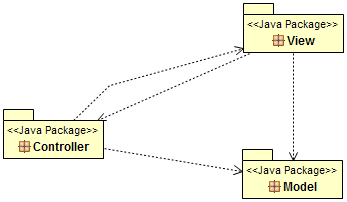
\includegraphics{Figures/retro_archi}
		\rule{35em}{0.5pt}
	\caption[Vue générale de l'application]{Vue générale de l'application}
\end{figure}

\subsection{Package model}
\subsubsection{Diagramme de classes rétro-générés}
\begin{figure}[H]
	\centering
		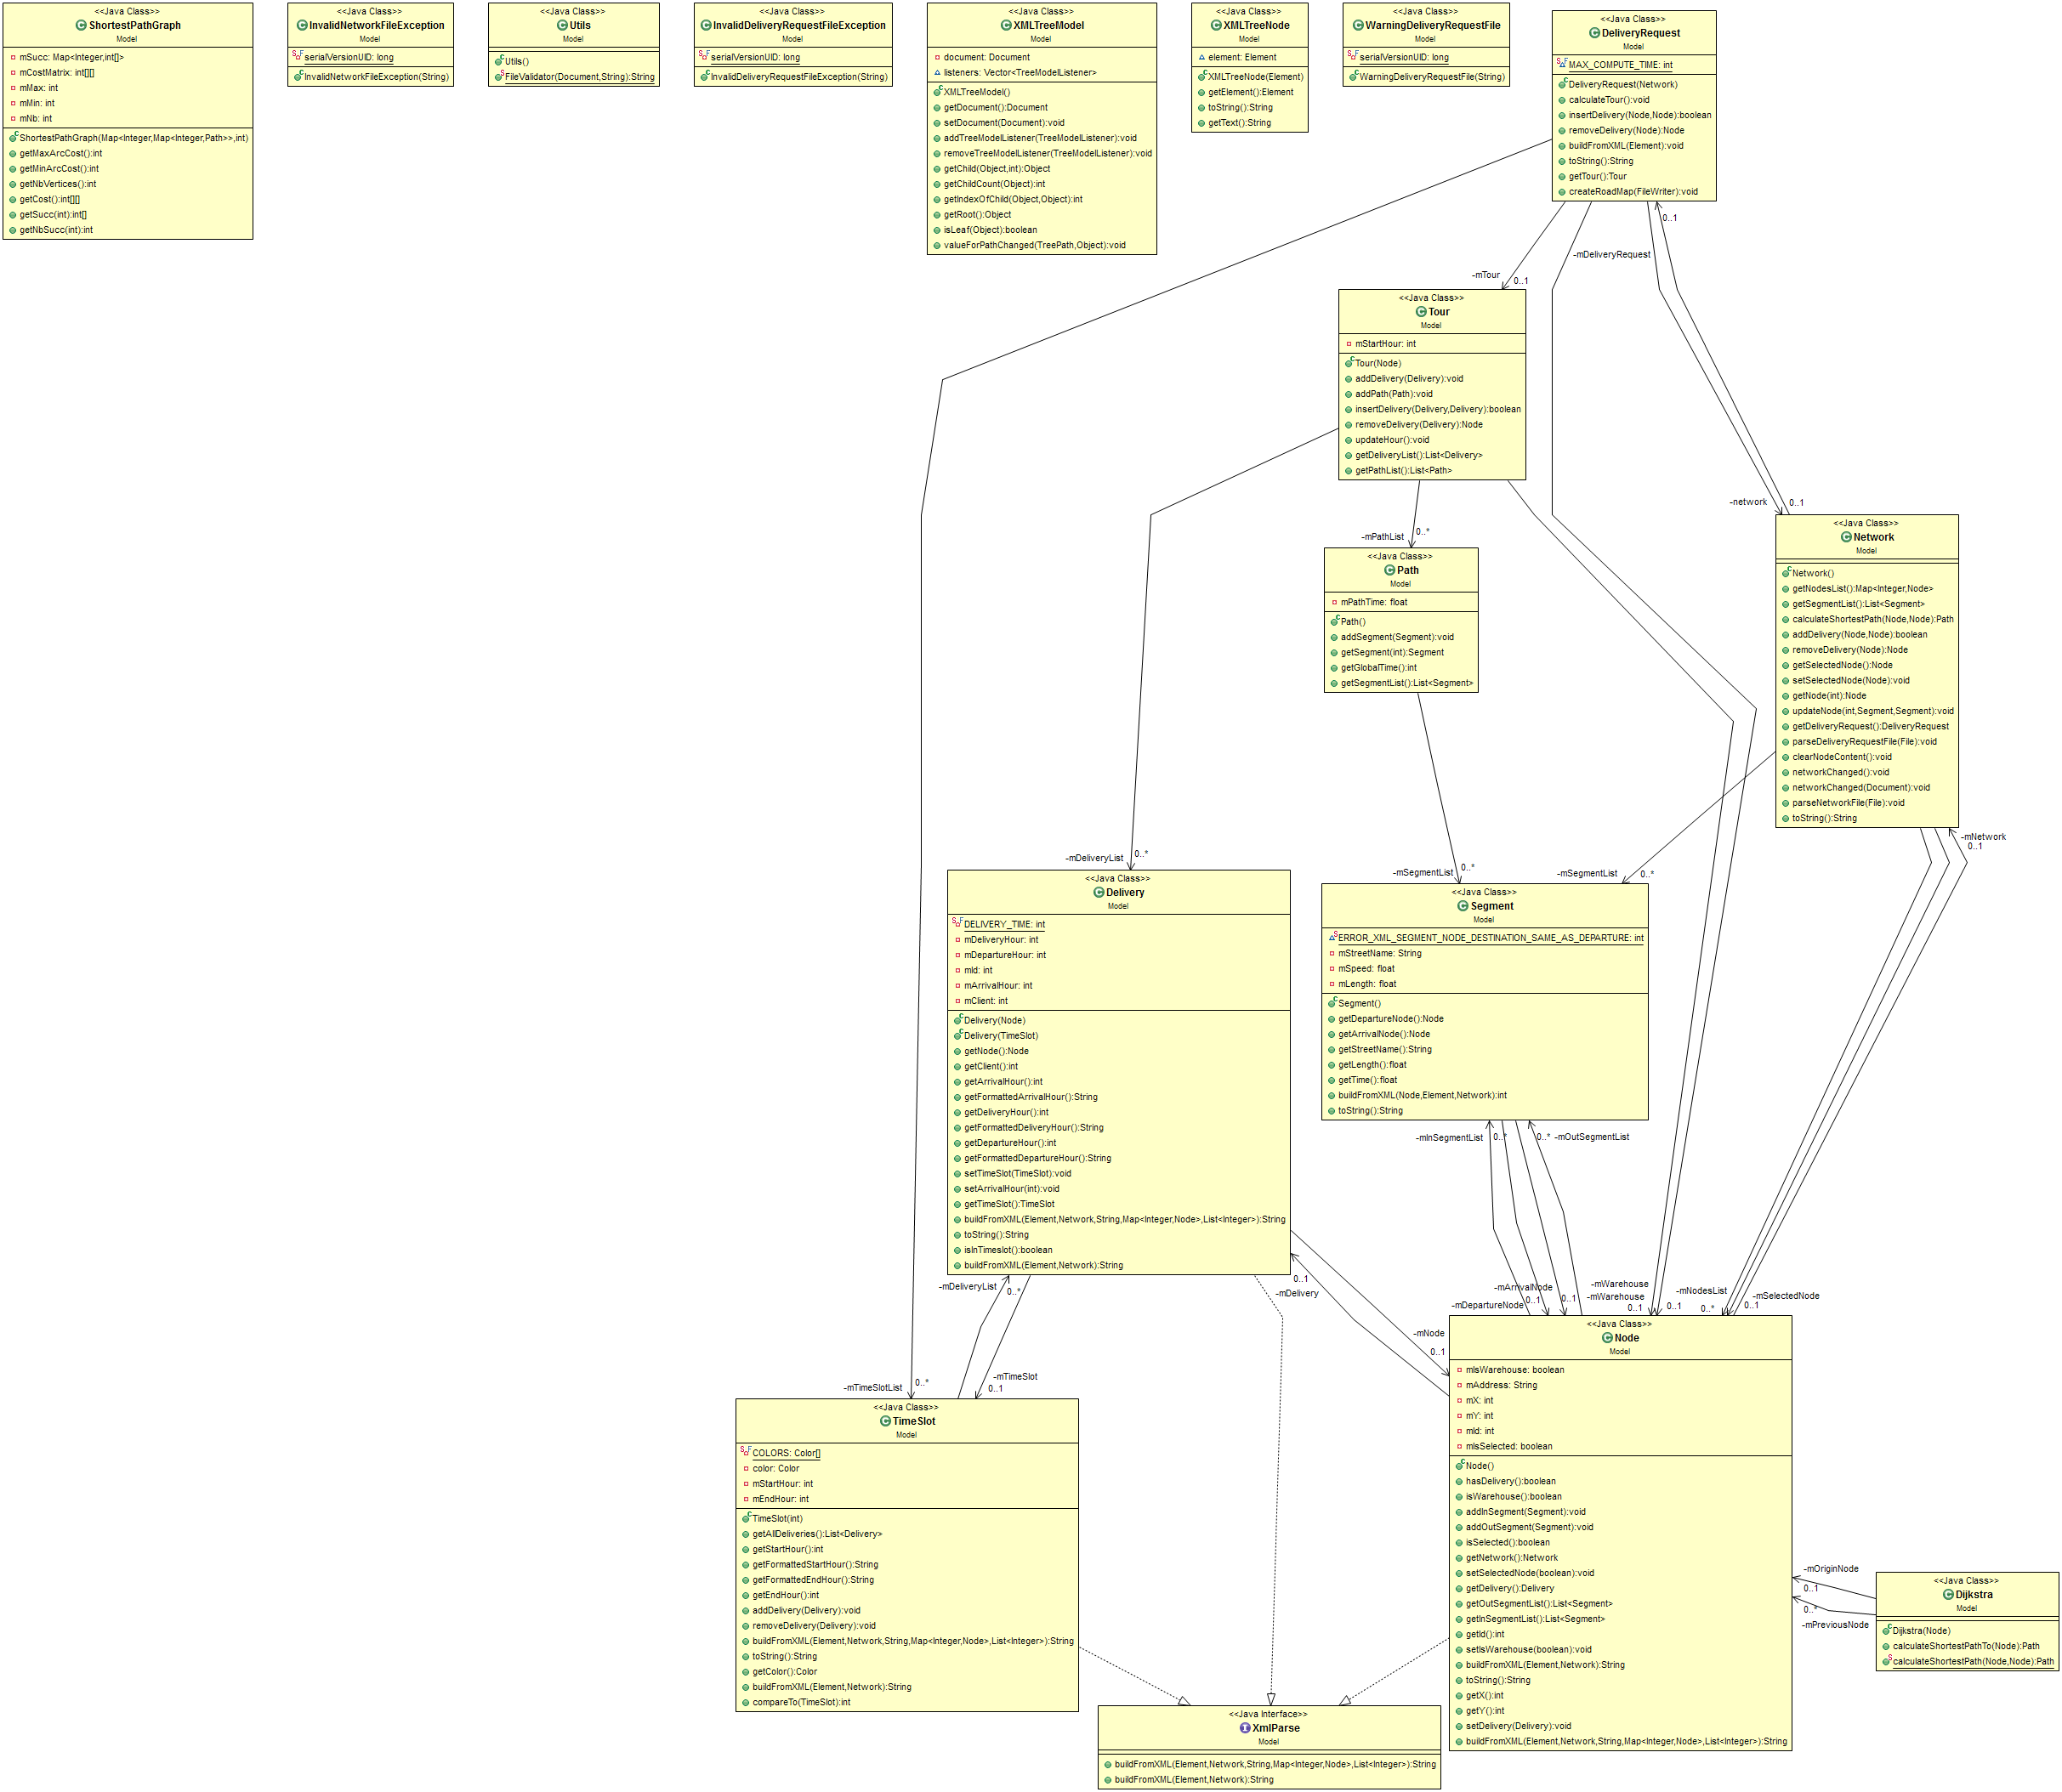
\includegraphics[width=\textwidth,height=\textheight,keepaspectratio]{Figures/retro_model}
		\rule{35em}{0.5pt}
	\caption[Diagramme de classes du package model]{Diagramme de classes du package model}
\end{figure}
\subsubsection{Dépendances}
\begin{figure}[H]
	\centering
		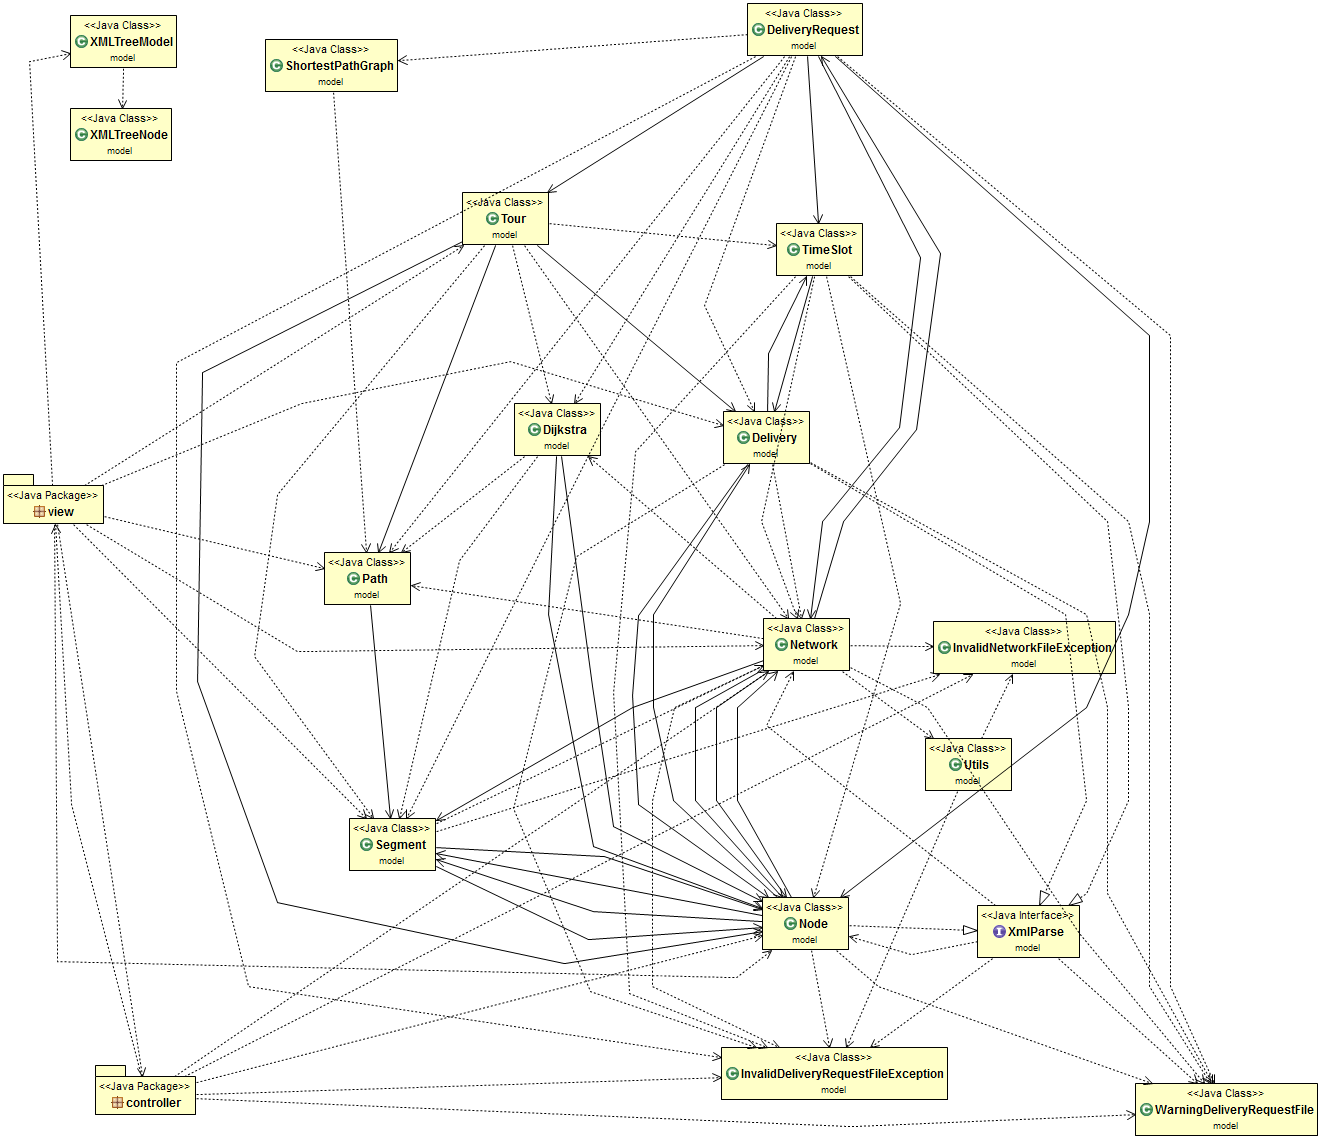
\includegraphics[width=\textwidth,height=\textheight,keepaspectratio]{Figures/retro_model_dep}
		\rule{35em}{0.5pt}
	\caption[Dépendances du package model]{Dépendances du package model}
\end{figure}

\subsection{Package view}
\subsubsection{Diagramme de classes rétro-générés}
\begin{figure}[H]
	\centering
		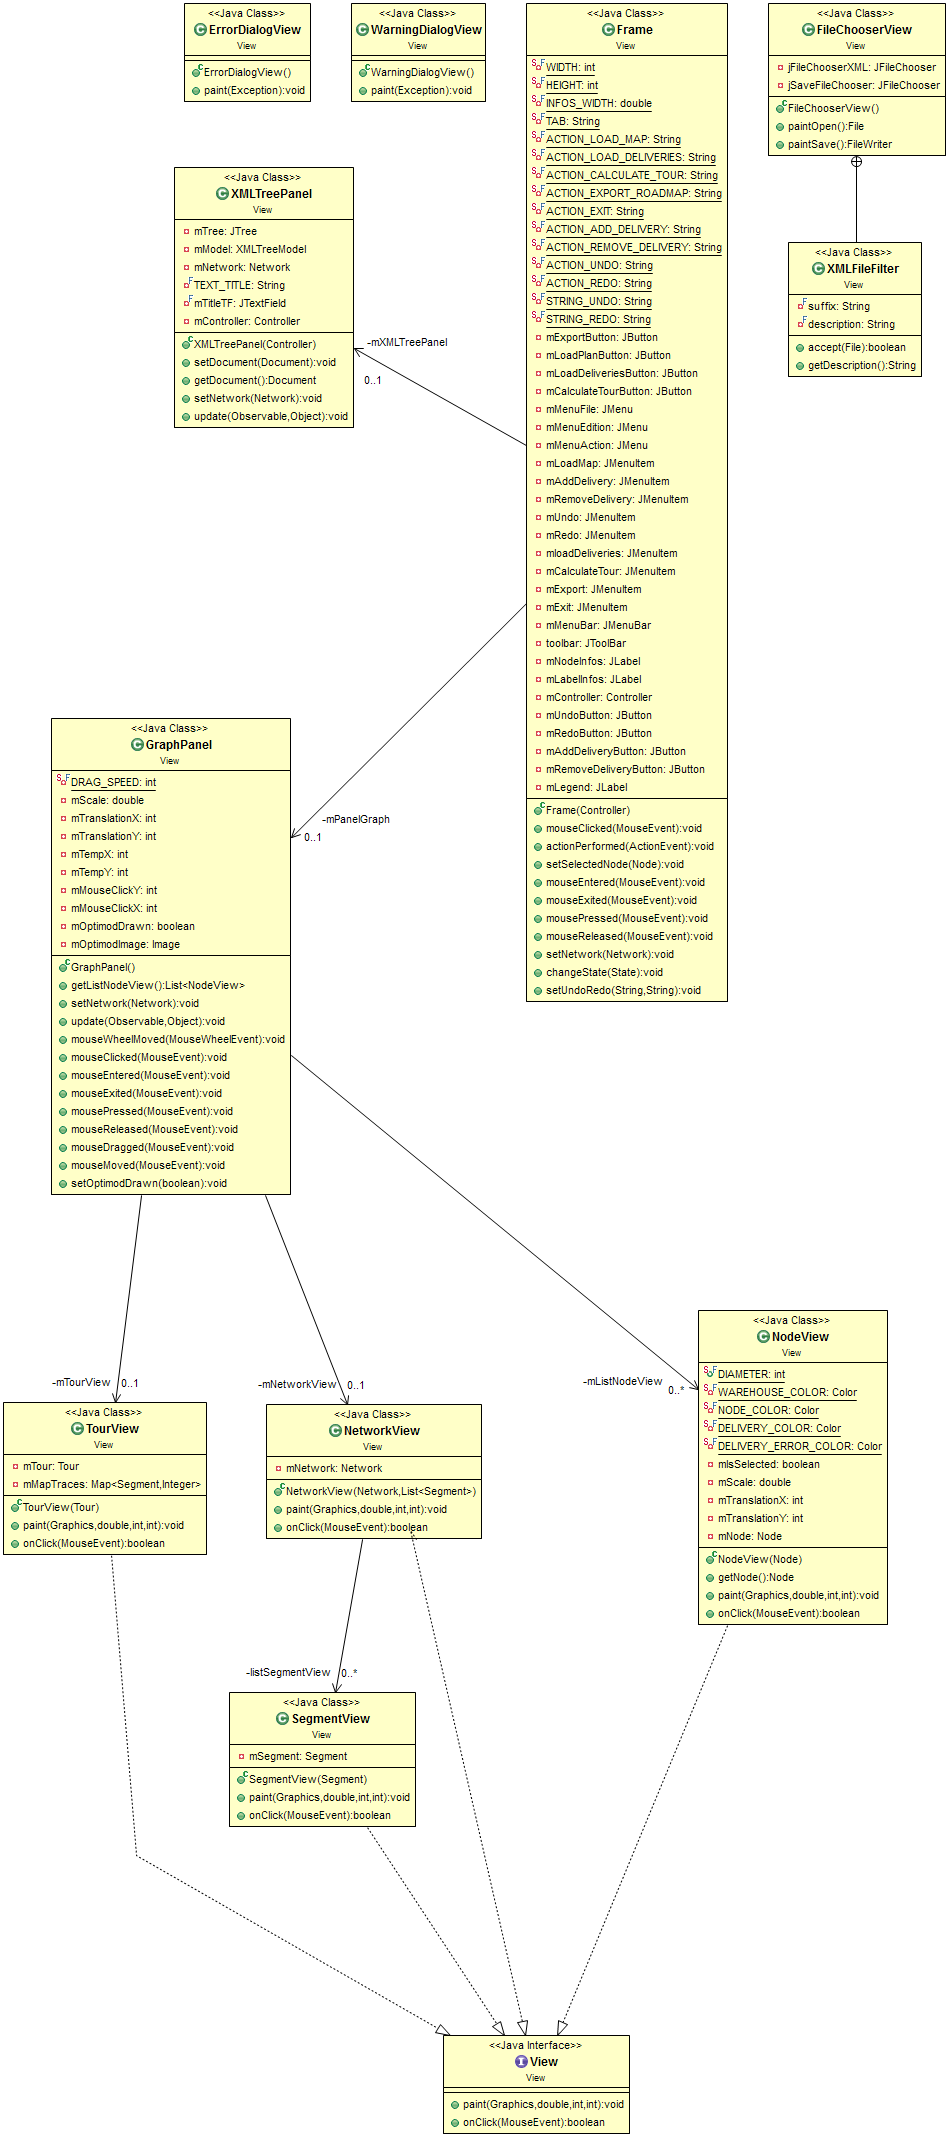
\includegraphics[width=\textwidth,height=\textheight,keepaspectratio]{Figures/retro_view}
		\rule{35em}{0.5pt}
	\caption[Diagramme de classes du package view]{Diagramme de classes du package view}
\end{figure}
\subsubsection{Dépendances}

\begin{figure}[H]
	\centering
		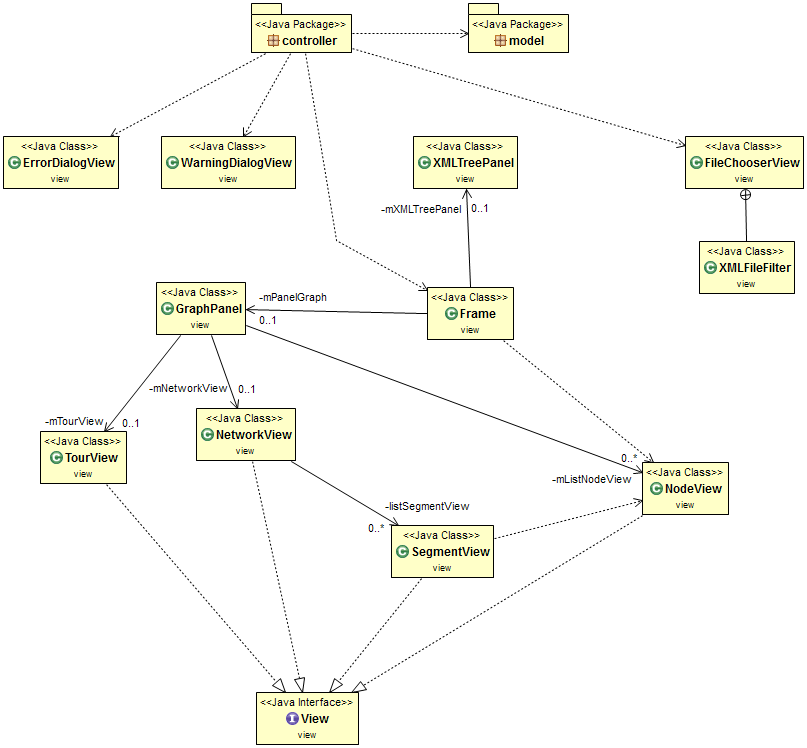
\includegraphics[width=\textwidth,height=\textheight,keepaspectratio]{Figures/retro_view_dep}
		\rule{35em}{0.5pt}
	\caption[Dépendances du package view]{Dépendances du package view}
\end{figure}


\subsection{Package Controller}
\subsubsection{Diagramme de classes rétro-générés}
\begin{figure}[H]
	\centering
		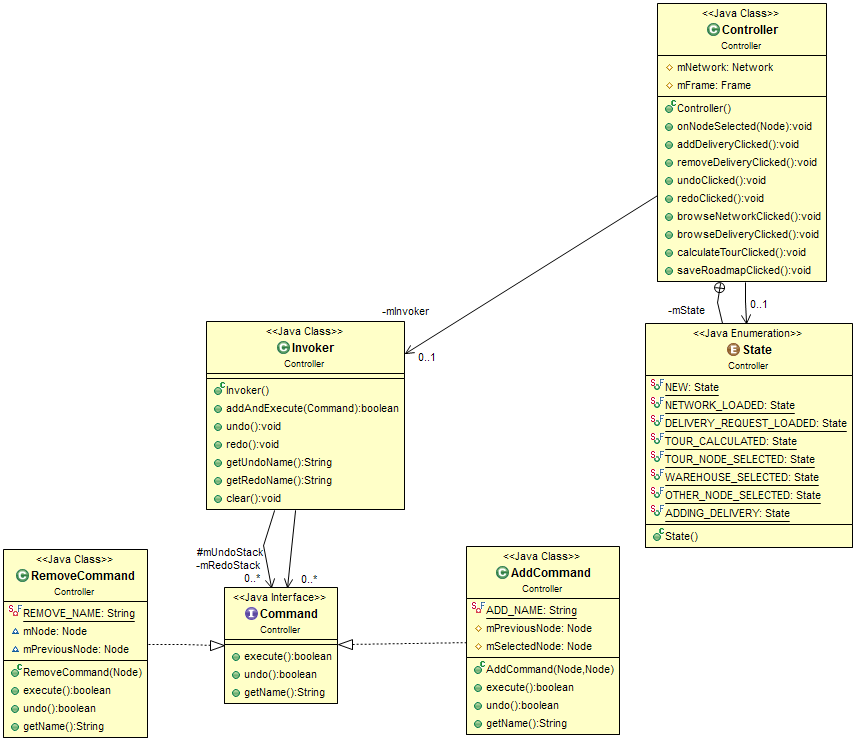
\includegraphics[width=\textwidth,height=\textheight,keepaspectratio]{Figures/retro_controller}
		\rule{35em}{0.5pt}
	\caption[Diagramme de classes du package controller]{Diagramme de classes du package controller}
\end{figure}
\subsubsection{Dépendances}

\begin{figure}[H]
	\centering
		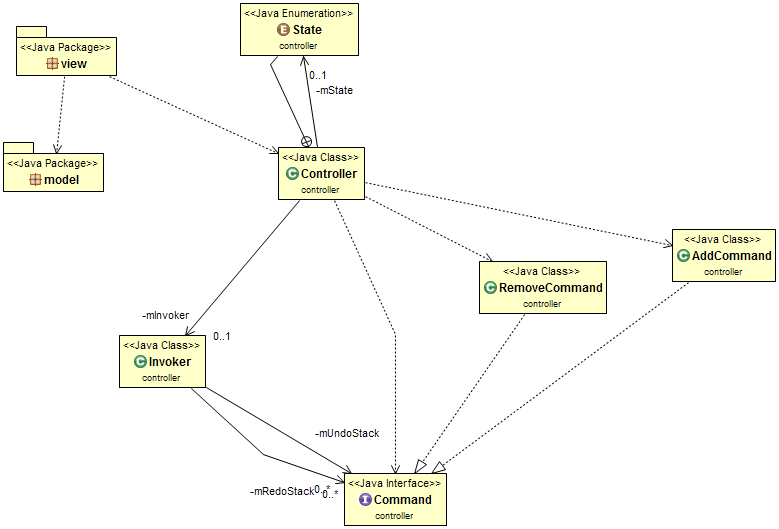
\includegraphics[width=\textwidth,height=\textheight,keepaspectratio]{Figures/retro_controller_dep}
		\rule{35em}{0.5pt}
	\caption[Dépendances du package controller]{Dépendances du package controller}
\end{figure}


%----------------------------------------------------------------------------------------
%	SECTION 2
%----------------------------------------------------------------------------------------

\section{Captures d'écran de l'application}

Sed ullamcorper quam eu nisl interdum at interdum enim egestas. Aliquam placerat justo sed lectus lobortis ut porta nisl porttitor. Vestibulum mi dolor, lacinia molestie gravida at, tempus vitae ligula. Donec eget quam sapien, in viverra eros. Donec pellentesque justo a massa fringilla non vestibulum metus vestibulum. Vestibulum in orci quis felis tempor lacinia. Vivamus ornare ultrices facilisis. Ut hendrerit volutpat vulputate. Morbi condimentum venenatis augue, id porta ipsum vulputate in. Curabitur luctus tempus justo. Vestibulum risus lectus, adipiscing nec condimentum quis, condimentum nec nisl. Aliquam dictum sagittis velit sed iaculis. Morbi tristique augue sit amet nulla pulvinar id facilisis ligula mollis. Nam elit libero, tincidunt ut aliquam at, molestie in quam. Aenean rhoncus vehicula hendrerit.